\chapter{Dynamiczna generacja terenu}

\section{System dynamicznego generowania terenu}

Często w opracowaniach zachodzi konieczność umieszczania różnego rodzaju zdjęć, wykresów, diagramów, algorytmów itp. różniących się jakością, rozmiarem oraz formatem zapisu grafiki. Różnice w elementach graficznych wynikające głownie z formatu zapisu mogę znacząco wpłynąć na jakość pracy. Korzystając z pakietu \LaTeX\ zaleca się, aby grafika umieszczana w opracowaniu zapisana była w formacie \textit{pdf} lub \textit{png}. Najwyższą jakość uzyskuję się zapisując elementy graficzne w formacie \textit{pdf}. Stosując ten format podczas skalowania elementu jego jakość graficzna będzie zawsze ta sama. Oczywiście pakiet \LaTeX\ wspiera również inne formaty zapisu, tj. \textit{jpg}, \textit{bmp}, itd.
\input{chapter4/2. System generowania biomów}

%=================================================================================================
% \section{Przykłady}
% Poniżej podano kilka przykładów umieszczania ilustracji w tekście.
% \begin{figure}[h!]
% 	\centering
% 		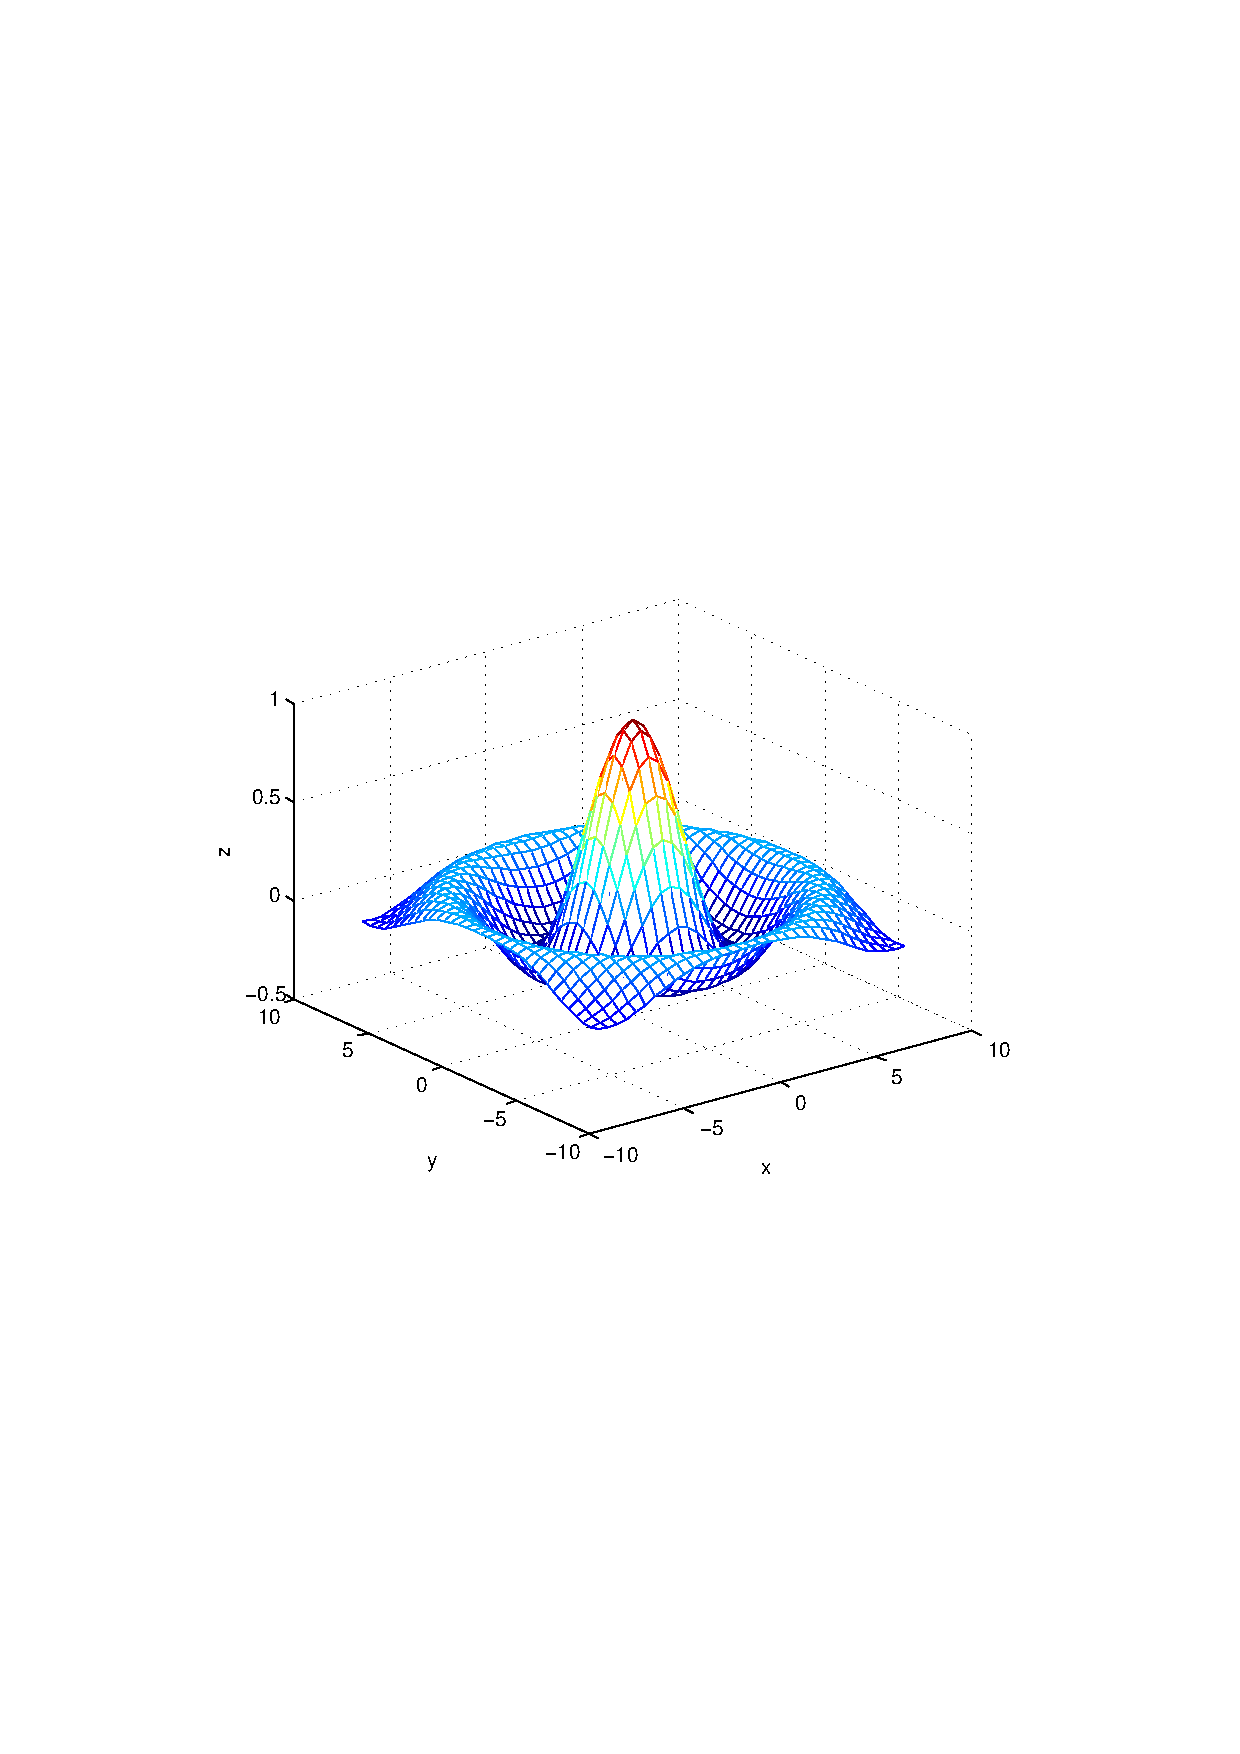
\includegraphics[width=12cm]{chapter4/img/sqrtsin.pdf}
% 		\label{fig:przyklad3D}
% 	\caption{Przykładowy wykres trójwymiarowy.}
% \end{figure}
% \newpage
% %-------------------------------------------------------------------------------------------------
% \begin{figure}[h!]
%   \centering
%   \subfloat[Wykres funkcji $\sin(x)$]{\label{fig:sinWyk}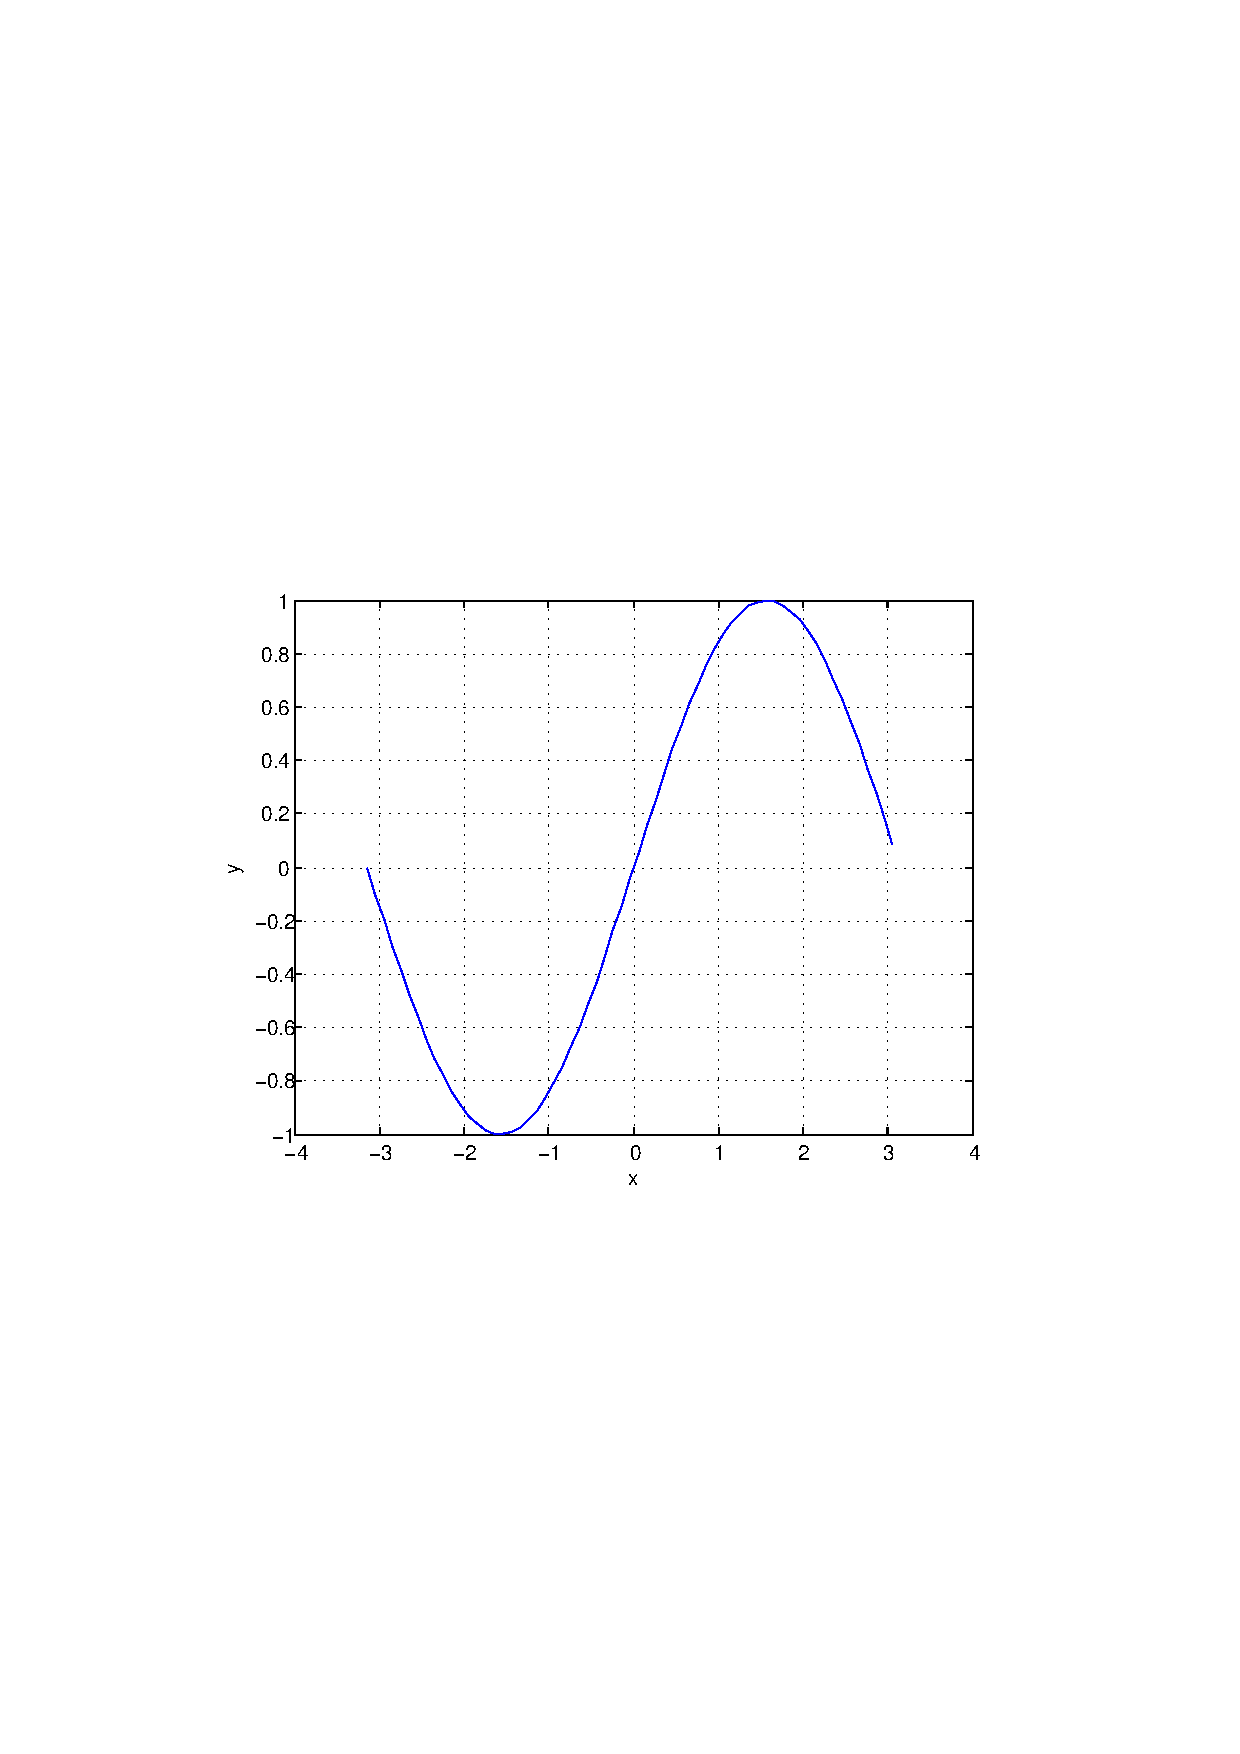
\includegraphics[width=0.45\textwidth]{chapter4/img/sin.pdf}}\quad
%   \subfloat[Wykres funkcji $\cos(x)$]{\label{fig:cosWyk}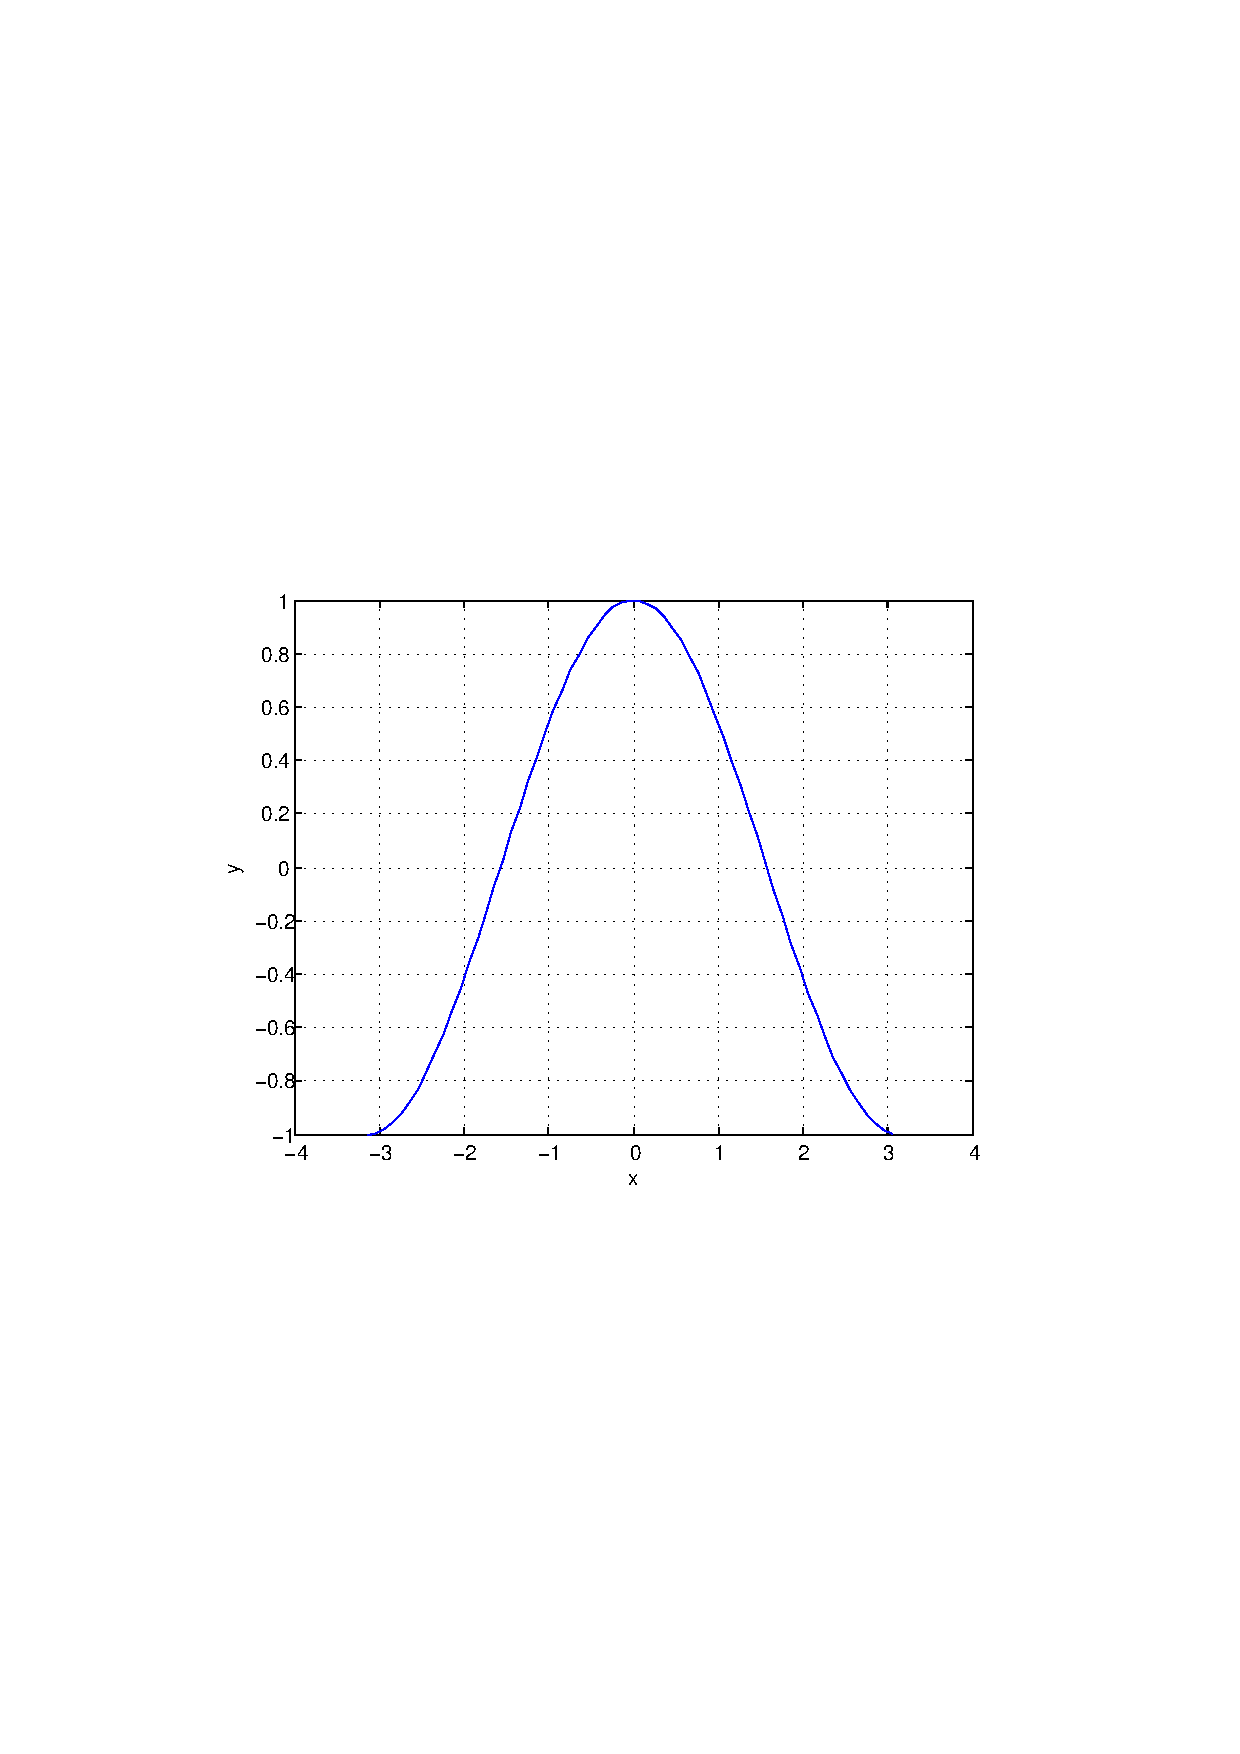
\includegraphics[width=0.45\textwidth]{chapter4/img/cos.pdf}}
%   \caption{Przykładowe wykresy funkcji $\sin (x)$ oraz $\cos (x)$ w przedziale $[-\pi, \pi]$.}
%   \label{fig:przyklad}
% \end{figure}
